\documentclass[12pt]{article}

\usepackage[margin=1in]{geometry}
\usepackage{fancyhdr}
\usepackage{amsmath, amsfonts, amsthm, amssymb, mathtools}  % Some math symbols
\usepackage{color}
% \usepackage{sectsty}
\usepackage{tcolorbox}
\usepackage{amsfonts}
\usepackage{titletoc}
\usepackage[normalem]{ulem}


\usepackage{hyperref}
\hypersetup{
    colorlinks,
    citecolor=black,
    filecolor=black,
    linkcolor=black,
    urlcolor=black
}


\titlecontents{section}[0em]
{\smallskip}
{\thecontentslabel\enspace}
{\hspace*{-5.3em}}
{\hfill\contentspage}



%%%%%%%%%%%% SETUP %%%%%%%%%%%%

% name of the class
\newcommand{\classname}{CSE 371}
% name of the assignment
\newcommand{\assignmentname}{HW1}
% collaborators on assignment
\newcommand{\collaborators}{Cameron Jennings}
\newcommand{\listcollaborators}{Collaborators: \collaborators}

\pagestyle{fancy}
\fancyhf{}
\setlength{\headheight}{13.59999pt}
\rhead{\thepage}
\lhead{\hyperref[beginning]{\classname \hspace{1em} \assignmentname}}

\usepackage{titlesec}
\titleformat{\subsection}{\normalfont\fontsize{12}{15}\bfseries}{\thesubsection}{1em}{}

\titleformat{\section}[block]
{\filcenter\large
\addtolength{\titlewidth}{2pc}%
\titleline*[c]{}%
\addvspace{6pt}%
}
{\thesection}{1em}{}
\titlespacing{\section}
{5pc}{*2}{*2}[5pc]


% \definecolor{WordSectionBlue}{RGB}{30, 90, 147}
% \allsectionsfont{\color{WordSectionBlue}}

%%%%%%%%%%%% FILE SPECIFIC IMPORTS %%%%%%%%%%%%

\usepackage{ragged2e}
\usepackage{tikz}

%%%%%%%%%%%%%%%%%%%%%%%%%%%%%%%%%%%%%%%%%%%%%%%

\renewcommand*{\thesection}{Question \arabic{section}.}
\renewcommand{\thesubsection}{(\alph{subsection})}

%%%%%%%%%%%% ENVIRONMENTS %%%%%%%%%%%%

\newenvironment{explanation}{\begin{tcolorbox}[colback=blue!2!white,colframe=blue!20!white]}{\end{tcolorbox}}

\newenvironment{subquestion}[1]{\subsection{#1}
\begin{tcolorbox}[colback=blue!2!white,colframe=blue!20!white]}{\end{tcolorbox}}

\newenvironment{sssq}[3]{\textbf{\thesubsubsection.\sssqARG{#1}} \hspace{0.5cm}
\begin{minipage}[t][\sssqARG{#2}][t]{14cm}
    \textbf{\sssqARG{#3}}
\end{minipage}
\begin{explanation}
}{\end{explanation}}

%%%%%%%%%%%% MY MACROS %%%%%%%%%%%%

\newcommand{\prob}{\mathbb{P}}
\newcommand{\expect}{\mathbb{E}}
\newcommand*\sssqARG{}
\newcommand{\bayes}{\textbf{Bayes' Theorem}}
\newcommand{\ltp}{\textbf{Law of Total Probability}}
\newcommand{\var}{\text{Var}}
\newcommand{\unif}{\sim \text{Unif}}
\newcommand{\expo}{\sim \text{Exponential}}
\newcommand{\caseif}{\text{if }}
\newcommand{\nlog}{\text{ln}}


%%%%%%%%%%%%%%%%%%%%%%%%%%%%%%%%%%%%%%
\begin{document}

    \setcounter{tocdepth}{1}
    \begin{center}\label{beginning}
        \tableofcontents 
    \end{center}

    \begin{center}
        \listcollaborators
    \end{center}

    % fix section heading font
    \titleformat{\section}{\normalfont\fontsize{17.28}{15}\bfseries\raggedright}{\thesection}{1em}{}
    \newpage
    \AddToHook{cmd/section/before}{\clearpage}

    % Question 1
    \section{}

        \begin{subquestion}{Draw out the state diagram of this circuit. Don't forget a reset state.}
            \begin{center}
                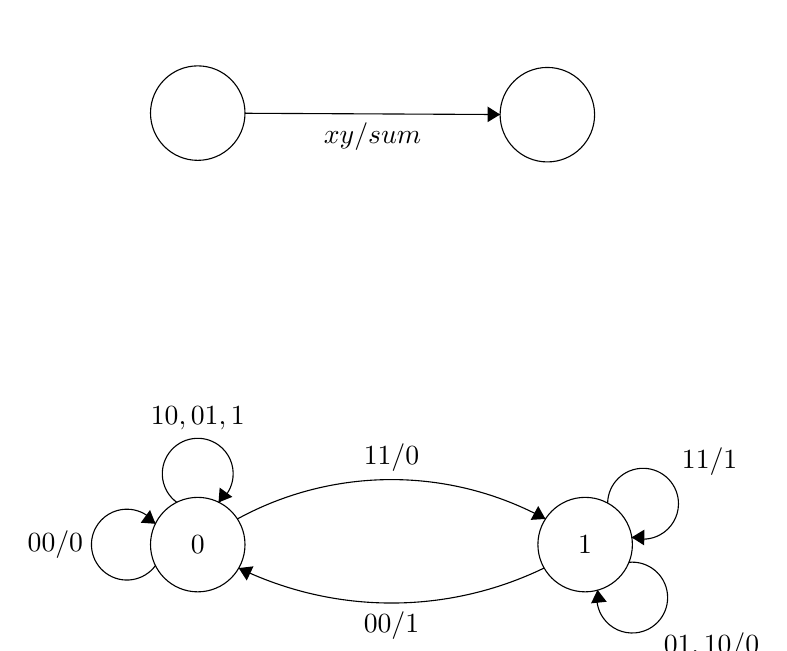
\begin{tikzpicture}[scale=0.2]
                \tikzstyle{every node}+=[inner sep=0pt]
                \draw [black] (27.4,-35.1) circle (3);
                \draw (27.4,-35.1) node {$0$};
                \draw [black] (52,-35.1) circle (3);
                \draw (52,-35.1) node {$1$};
                \draw [black] (27.4,-7.7) circle (3);
                \draw [black] (49.6,-7.8) circle (3);
                \draw [black] (30.4,-7.71) -- (46.6,-7.79);
                \fill [black] (46.6,-7.79) -- (45.8,-7.28) -- (45.8,-8.28);
                \draw (38.5,-8.27) node [below] {$xy/sum$};
                \draw [black] (24.72,-36.423) arc (324:36:2.25);
                \draw (20.15,-35.1) node [left] {$00/0$};
                \fill [black] (24.72,-33.78) -- (24.37,-32.9) -- (23.78,-33.71);
                \draw [black] (26.077,-32.42) arc (234:-54:2.25);
                \draw (27.4,-27.85) node [above] {$10,01,1$};
                \fill [black] (28.72,-32.42) -- (29.6,-32.07) -- (28.79,-31.48);
                \draw [black] (29.917,-33.472) arc (118.68555:61.31445:20.382);
                \fill [black] (49.48,-33.47) -- (49.02,-32.65) -- (48.54,-33.53);
                \draw (39.7,-30.47) node [above] {$11/0$};
                \draw [black] (53.427,-32.474) arc (179.21759:-108.78241:2.25);
                \draw (58.11,-29.84) node [right] {$11/1$};
                \fill [black] (54.95,-34.64) -- (55.75,-35.15) -- (55.76,-34.15);
                \draw [black] (49.396,-36.586) arc (-64.1509:-115.8491:22.239);
                \fill [black] (30,-36.59) -- (30.51,-37.38) -- (30.94,-36.48);
                \draw (39.7,-39.31) node [below] {$00/1$};
                \draw [black] (54.768,-36.225) arc (95.61572:-192.38428:2.25);
                \draw (60.02,-40.64) node [below] {$01,10/0$};
                \fill [black] (52.79,-37.98) -- (52.37,-38.83) -- (53.37,-38.73);
                \end{tikzpicture}
                \end{center}
        \end{subquestion}

        \begin{subquestion}{Implement modules \texttt{hw1p1} and \texttt{hw1p1\_tb}, which thoroughly simulates an instance of called dut.}
        % \begin{subquestion}{Implement modules , which thoroughly simulates an instance of called dut.}
            Implemented in SystemVerilog, submitted on gradescope
        \end{subquestion}

    % Question 2
    \section{}
        \begin{subquestion}{Implement modules \texttt{hw1p2} and \texttt{hw1p2\_tb} which thoroughly simulates an instance of hw1p2 called dut.}
            Implemented in SystemVerilog
            
        \end{subquestion}

    % Question 3
    \section{}
        \begin{subquestion}{Draw out the state diagram for the FSM}
            \begin{center}
                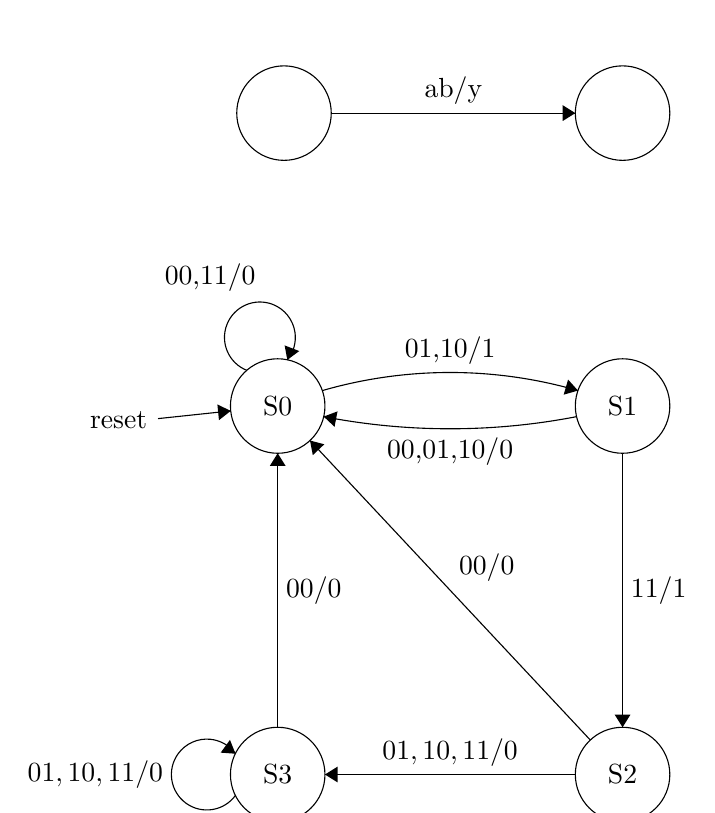
\begin{tikzpicture}[scale=0.2]
                    \tikzstyle{every node}+=[inner sep=0pt]
                    \draw [black] (25.5,-8.1) circle (3);
                    \draw [black] (47,-8.1) circle (3);
                    \draw [black] (25.1,-26.7) circle (3);
                    \draw (25.1,-26.7) node {S0};
                    \draw [black] (47,-26.7) circle (3);
                    \draw (47,-26.7) node {S1};
                    \draw [black] (25.1,-50.1) circle (3);
                    \draw (25.1,-50.1) node {S3};
                    \draw [black] (47,-50.1) circle (3);
                    \draw (47,-50.1) node {S2};
                    \draw [black] (28.5,-8.1) -- (44,-8.1);
                    \fill [black] (44,-8.1) -- (43.2,-7.6) -- (43.2,-8.6);
                    \draw (36.25,-7.6) node [above] {ab/y};
                    \draw [black] (17.5,-27.5) -- (22.12,-27.01);
                    \draw (16.85,-27.6) node [left] {reset};
                    \fill [black] (22.12,-27.01) -- (21.27,-26.6) -- (21.37,-27.6);
                    \draw [black] (23.147,-24.438) arc (248.53446:-39.46554:2.25);
                    \draw (20.81,-19.44) node [above] {00,11/0};
                    \fill [black] (25.71,-23.77) -- (26.47,-23.21) -- (25.54,-22.85);
                    \draw [black] (27.934,-25.72) arc (106.12905:73.87095:29.215);
                    \fill [black] (44.17,-25.72) -- (43.54,-25.02) -- (43.26,-25.98);
                    \draw (36.05,-24.07) node [above] {01,10/1};
                    \draw [black] (44.078,-27.375) arc (-79.03654:-100.96346:42.209);
                    \fill [black] (28.02,-27.37) -- (28.71,-28.02) -- (28.9,-27.04);
                    \draw (36.05,-28.65) node [below] {00,01,10/0};
                    \draw [black] (47,-29.7) -- (47,-47.1);
                    \fill [black] (47,-47.1) -- (47.5,-46.3) -- (46.5,-46.3);
                    \draw (47.5,-38.4) node [right] {11/1};
                    \draw [black] (44.95,-47.91) -- (27.15,-28.89);
                    \fill [black] (27.15,-28.89) -- (27.33,-29.82) -- (28.06,-29.13);
                    \draw (36.58,-36.93) node [right] {$00/0$};
                    \draw [black] (44,-50.1) -- (28.1,-50.1);
                    \fill [black] (28.1,-50.1) -- (28.9,-50.6) -- (28.9,-49.6);
                    \draw (36.05,-49.6) node [above] {$01,10,11/0$};
                    \draw [black] (22.42,-51.423) arc (324:36:2.25);
                    \draw (17.85,-50.1) node [left] {$01,10,11/0$};
                    \fill [black] (22.42,-48.78) -- (22.07,-47.9) -- (21.48,-48.71);
                    \draw [black] (25.1,-47.1) -- (25.1,-29.7);
                    \fill [black] (25.1,-29.7) -- (24.6,-30.5) -- (25.6,-30.5);
                    \draw (25.6,-38.4) node [right] {$00/0$};
                \end{tikzpicture}
            \end{center}
        \end{subquestion}

    \section{Sketch the hardware each circuit implies}
        \begin{subquestion}{Circuit 1 Parallel}
            \begin{center}
                \includegraphics[scale=0.8]{Images/Question 4 Circuit 1 Parallel.pdf}
            \end{center}
            
        \end{subquestion}

        \begin{subquestion}{Circuit 1 Sequential}
            \begin{center}
                \includegraphics[scale=0.9]{Images/Question 4 Circuit 1 Sequential.pdf}
            \end{center}
            
        \end{subquestion}

        \begin{subquestion}{Circuit 2 Parallel}
            \begin{center}
                \includegraphics[scale=0.8]{Images/Question 4 Circuit 2 Parallel.pdf}
            \end{center}
            
        \end{subquestion}

        \begin{subquestion}{Circuit 2 Sequential}
            \begin{center}
                \includegraphics[scale=0.8]{Images/Question 4 Circuit 2 Parallel.pdf}
            \end{center}
            
        \end{subquestion}

    
\end{document}
